This appendix provides a brief tutorial for the \julia\ package. We release this package on GitHub with the name \siplibjl.

\subsection{Prerequisites}
We assume that you are in Linux environment. To use \siplibjl, you need to perform the following steps:
\begin{enumerate}
	\item Download $\julia\ge 0.6.2$ and set up.
	\item Install \julia\ packages: \texttt{Distributions.jl}, \texttt{StructJuMP.jl}, \texttt{PyPlot.jl} by executing
	\begin{itemize}
		\item \texttt{Pkg.add("Distributions")}
		\item \texttt{Pkg.add("StructJuMP")}
		\item \texttt{Pkg.add("PyPlot")}
	\end{itemize}
	Then, execute \texttt{Pkg.update()} to make them up-to-date.
	\item Download and place the \siplibjl\ package to any directory (say \texttt{dir}) in your computer
	\item Open a terminal and change working directory to \texttt{dir/Siplib/src/}:
	\begin{itemize}
		\item \texttt{cd dir/Siplib/src}	
	\end{itemize}
	\item Run \julia\ in that directory
	\item Excute \texttt{include("Siplib.jl")}
	\item Excute \texttt{using Siplib}
\end{enumerate}
Then, you are all set to use \siplibjl. To make it sure, execute the following line to generate DCAP\_2\_2\_2\_10 instance:
\begin{lstlisting}[frame=single,language=julia]
julia> generateSMPS(:DCAP, [2,2,2,10])
\end{lstlisting}
If it works well, you will see the three files in \texttt{dir/Siplib/instance}:
\begin{itemize}
	\item DCAP\_2\_2\_2\_10.cor
	\item DCAP\_2\_2\_2\_10.tim
	\item DCAP\_2\_2\_2\_10.sto
\end{itemize}


\subsection{Basic usages}
\subsubsection{Generating \smps\ or \mps\ instance}
Use \texttt{generateSMPS(problem, params\_arr)} or \texttt{generateMPS(problem, params\_arr)} with proper values in Table \ref{table:numparameter} to generate \smps\ or \mps\ files for instances, for example:
\begin{lstlisting}[frame=single,language=julia]
julia> generateSMPS(:DCAP, [2,2,2,10])
\end{lstlisting}
The default directory in which the files are stored is \texttt{dir/Siplib/instance}. You can change the directory by specifying explicit path:
\begin{lstlisting}[frame=single,language=julia]
julia> generateSMPS(:DCAP, [2,2,2,10], "another/directory")
\end{lstlisting}
\texttt{generateSMPS()} has four keyword arguments: \texttt{genericnames}, \texttt{seed}, \texttt{splice}, and \texttt{lprelax}. \texttt{generateMPS()} has the same four keyword arguments with one more keyword argument \texttt{decfile}. If we set \texttt{decfile=true}, a .dec file that specifies scenario-specific blocks is generated together. For more details, please see the later subsection (\ref{tutorial:gen_instance}).

\begin{table}[H]
	\centering
	\resizebox{\textwidth}{!}{%
		\begin{threeparttable}
			\caption{Acceptable values for \texttt{problem} and \texttt{params\_arr} arguments pairs}
			\label{table:numparameter}
			\begin{tabular}{@{}ccl@{}}
				\toprule
				\texttt{problem}  & \texttt{params\_arr}     & Remark                                                                                                                                     \\ \midrule
				\texttt{:AIRLIFT}              & \texttt{[$\mathcal{S}$]}          & Integer $\mathcal{S}$.                                                                                   \\
				\texttt{:CARGO}              & \texttt{[$\mathcal{S}$]}          & Integer $\mathcal{S}$.                                                                                   \\
				\texttt{:CHEM}              & \texttt{[$\mathcal{S}$]}          & Integer $\mathcal{S}$.                                                                                   \\								
				\texttt{:DCAP}               & \texttt{[R, T, N, $\mathcal{S}$]} & All parameters are integer.                                                                                                                \\
				\texttt{:MPTSPs}             & \texttt{[d, N, $\mathcal{S}$]}    & String $\texttt{d}\in \{\mathrm{``D0"}, \mathrm{``D1"}, \mathrm{``D2"}, \mathrm{``D3"}\}$. All other parameters are integer.                                                              \\
				\texttt{:PHONE}              & \texttt{[$\mathcal{S}$]}          & Integer $\mathcal{S}$.                                                                                   \\
				\texttt{:SDCP}                & \texttt{[k, p, d, $\mathcal{S}$]}       & \multicolumn{1}{l}{Integer \texttt{k}. Percentage $\texttt{p}\in [0.0,100.0]$.  Integer $\mathcal{S}\le 1000$.}                                             \\
				\multicolumn{1}{l}{}         & \multicolumn{1}{l}{}            & \multicolumn{1}{r}{String $\texttt{d}\in \{\mathrm{``FallWD"}, \mathrm{``FallWE"}, \mathrm{``WinterWD"}, \mathrm{``WinterWE"}, \mathrm{``SpringWD"}, \mathrm{``SpringWE"}, \mathrm{``SummerWD"}, \mathrm{``SummerWE"} \}.$}\\				
				\texttt{:SIZES}              & \texttt{[$\mathcal{S}$]}          & Integer $\mathcal{S}$.                                                                                   \\
				\texttt{:SMKP}               & \texttt{[I, $\mathcal{S}$]}       & All parameters are integer.                                                                                                                \\
				\texttt{:SSLP}               & \texttt{[I, J, $\mathcal{S}$]}    & All parameters are integer.                                                                                                                \\
				\texttt{:SUC}                & \texttt{[d, $\mathcal{S}$]}       & \multicolumn{1}{l}{Integer $\mathcal{S}\le 1000$.}                                             \\
				\multicolumn{1}{l}{}         & \multicolumn{1}{l}{}            & \multicolumn{1}{r}{String $\texttt{d}\in \{\mathrm{``FallWD"}, \mathrm{``FallWE"}, \mathrm{``WinterWD"}, \mathrm{``WinterWE"}, \mathrm{``SpringWD"}, \mathrm{``SpringWE"}, \mathrm{``SummerWD"}, \mathrm{``SummerWE"} \}.$}\\				
				\bottomrule
			\end{tabular}
			\begin{tablenotes}
				\item Note: $\mathcal{S}$ is always the number of scenarios.
			\end{tablenotes}
		\end{threeparttable}
	}
\end{table}

\subsubsection{Solving an instance and calculating its bounds}
First, use \texttt{getModel(problem, params\_arr)} to construct a \jumpmodel\ object of an instance. For example:
\begin{lstlisting}[frame=single,language=julia]
julia> m = getModel(:DCAP, [2,2,2,10])
\end{lstlisting}
Then, use \texttt{RP(model, solver)}, \texttt{WS(model, solver)}, and \texttt{EEV(model, solver)} with including any solver (e.g., \texttt{using CPLEX}) to solve the instance in three different ways:
\begin{lstlisting}[frame=single,language=julia]
julia> using CPLEX
julia> RP(m, CplexSolver())
julia> WS(m, CplexSolver())
julia> EEV(m, CplexSolver())
\end{lstlisting}
Detailed definitions for RP, WS, and EEV are found in Section \ref{subsec:sol_report}.

\subsubsection{Plotting sparsity}
Use \texttt{generateSparsityPlots(problem, params\_arr)} to generate and save the sparsity plots. Excute the following lines:
\begin{lstlisting}[frame=single,language=julia]
julia> generateSparsityPlots(:DCAP, [2,2,2,10])
\end{lstlisting}
The default directory in which the plots are stored is \texttt{dir/Siplib/plot}. You can change the directory by specifying explicit path:
\begin{lstlisting}[frame=single,language=julia]
julia> generateSparsityPlots(:DCAP, [2,2,2,10], "another/directory")
\end{lstlisting}
For details, please see the later subsection (\ref{tutorial:analyze_instance}).
\subsubsection{Reporting size and sparsity}
Use \texttt{getSize(problem, params\_arr)} and \texttt{getSparsity(problem, params\_arr)} to get the size and sparsity information. Excute the following lines to construct objects that contain the information:
\begin{lstlisting}[frame=single,language=julia]
julia> size = getSize(:DCAP, [2,2,2,10])
julia> sparsity = getSparsity(:DCAP, [2,2,2,10])
\end{lstlisting}
For details, please see the later subsection (\ref{tutorial:analyze_instance}).

\subsection{Generating instances} \label{tutorial:gen_instance}
\siplibjl\ provides four functions with regard to instance generation:
\begin{itemize}
	\item \texttt{getInstanceName()}
	\item \texttt{getModel()}
	\item \texttt{writeSMPS()}
	\item \texttt{generateSMPS()}
\end{itemize}
In short, \texttt{getInstanceName()} returns a \texttt{String}-type instance name, \texttt{getModel()} constructs \jumpmodel-type object, \texttt{writeSMPS()} converts a \jumpmodel-type object to the three \smps\ files, and \texttt{generateSMPS()} does both \texttt{getModel()} and \texttt{writeSMPS()} simultaneously.
\subsubsection{function \texttt{getInstanceName()}}
\begin{lstlisting}[frame=single,language=julia]
function getInstanceName(problem::Symbol, params_arr::Any)::String
\end{lstlisting}		
The function \texttt{getInstanceName()} is an utility function that returns a \texttt{String}-type instance name defined in Table \ref{table:naming_rule}. It takes two necessary input arguments \texttt{problem} and \texttt{params\_arr}:
\begin{quote}
	\noindent\underline{\texttt{problem}} (necessary, positional) The \texttt{Symbol}-type argument that specify the problem of which we want to generate instance. The appropriate values are given in Table \ref{table:numparameter}. 
\end{quote}

\begin{quote}
	\noindent\underline{\texttt{params\_arr}} (necessary, positional) The argument that specifies the parameters of the problem. It must be properly paired with the argument \texttt{problem}. The appropriate values are given in Table \ref{table:numparameter}. 
\end{quote}

\subsubsection{function \texttt{getModel()}} 
\begin{lstlisting}[frame=single,language=julia]
function getModel(problem::Symbol, params_arr::Any ; seed::Int=1, lprelax::Int=0)::JuMP.Model
\end{lstlisting}

The function \texttt{getModel()} returns a \jumpmodel-type object. It has two necessary positional arguments and two optional keyword arguments:
\begin{quote}
	\noindent\underline{\texttt{problem}} (necessary, positional) The \texttt{Symbol}-type argument that specify the problem of which we want to generate instance. The appropriate values are given in Table \ref{table:numparameter}. 
\end{quote}

\begin{quote}
	\noindent\underline{\texttt{params\_arr}} (necessary, positional) The argument that specifies the parameters of the problem. It must be properly paired with the argument \texttt{problem}. The appropriate values are given in Table \ref{table:numparameter}. 
\end{quote}

\begin{quote}
	\noindent\underline{\texttt{seed}} (optional, keyword) The integer argument \texttt{seed} specifies the seed of pseudo-random number generator in \julia. If specific value is not supplied, \texttt{seed=1} as a default.
\end{quote}

\begin{quote}
	\noindent\underline{\texttt{lprelax}} (optional, keyword) The keyword argument specifying the level of LP-relaxation of an instance. Table \ref{table:lprelax} summarizes the acceptable values with its meaning. If not specified, \texttt{lprelax=0} as a default which means no LP-relaxation.
\end{quote}

\begin{table}[H]
	\centering
	\caption{Acceptable values for \texttt{lprelax} argument}
	\label{table:lprelax}
	%\resizebox{\textwidth}{!}{%
	\begin{tabular}{@{}ll@{}}
		\toprule
		\texttt{lprelax} & Remark                                            \\ \midrule
		$0$ (default)              & No LP-relaxation                                  \\
		$1$              & First-stage only LP-relaxation                    \\
		$2$              & Second-stage only LP-relaxation                   \\
		$3$              & Full LP-relaxation (both first-stage and second-stage) \\ \bottomrule
	\end{tabular}%
	%	}
\end{table}

For example, executing the following line constructs a \jumpmodel\ object \texttt{model} of instance DCAP\_3\_4\_2\_100 with default random seed 1 and without LP-relaxation.
\begin{lstlisting}[frame=single,language=julia]
julia> model = getModel(:DCAP, [3,4,2,100])
\end{lstlisting}
The keyword argument \texttt{seed} can be changed by another value, for example,
\begin{lstlisting}[frame=single,language=julia]
julia> model = getModel(:DCAP, [3,4,2,100], seed=2)
\end{lstlisting}
The line below constructs a \jumpmodel\ object of the second-stage only LP-relaxed instance DCAP\_3\_4\_2\_100 using a different random seed 2.
\begin{lstlisting}[frame=single,language=julia]
julia> model = getModel(:DCAP, [3,4,2,100], seed=2, lprelax=2)
\end{lstlisting}




\subsubsection{function \texttt{writeSMPS()}} 
\begin{lstlisting}[frame=single,language=julia]
function writeSMPS(model::JuMP.Model, INSTANCE_NAME::String="instance", DIR_NAME::String="$(dirname(@__FILE__))/../instance"; genericnames::Bool=true, splice::Bool=true)
\end{lstlisting}
The function \texttt{writeSMPS()} converts a \jumpmodel\ object to \smps\ files. It takes up to five inputs:

\begin{quote}
	\noindent\underline{\texttt{model}} (necessary, positional) The \jumpmodel-type object of which we want to generate \smps\ files.
\end{quote}

\begin{quote}
	\noindent\underline{\texttt{INSTANCE\_NAME}} (optional, positional) The \texttt{String}-type argument that will be the name of \smps\ files. If not specified, \texttt{INSTANCE\_NAME="instance"} as a default. Then, the three files are generated:
	\begin{itemize}
		\item instance.cor
		\item instance.tim
		\item instance.sto
	\end{itemize}
\end{quote}

\begin{quote}
	\noindent\underline{\texttt{DIR\_NAME}} (optional, positional) The \texttt{String}-type argument to indicate a directory where the files are stored. The \smps\ files are stored in the default folder ``\texttt{$\sim$/Siplib/instance/}'' unless the argument \texttt{DIR\_NAME} is specified.
\end{quote}

\begin{quote}
	\noindent\underline{\texttt{genericnames}} (optional, keyword) The \texttt{Bool}-type keyword argument that decides whether or not we keep the original variable names. 
	
	If \texttt{genericnames=true}, \smps\ files are written with the variable names \texttt{VAR1}, \texttt{VAR2}, \texttt{VAR3}, and so on. If \texttt{genericnames=false}, the original variable names such as \texttt{x[1,1]}, \texttt{y[2,2]}, and \texttt{z[3,3]} are maintained. \texttt{true} as a default.
\end{quote}

\begin{quote}
	\noindent\underline{\texttt{splice}} (optional, keyword) The \texttt{Bool}-type keyword argument that decides whether or not the stochastic data stored in the \jumpmodel-type object is spliced after writing the \smps\ files. Hence, it increases the memory efficiency during the generation of \smps\ files. However, the spliced \jumpmodel-type object cannot be re-used for further purpose. \texttt{true} as a default.
\end{quote}

Executing the following lines store the three \smps\ files of DCAP\_3\_4\_2\_100 in the default directory ``\texttt{$\sim$/Siplib/instance/}''  with the default file name ``instance'', generic variable names, and splicing stored data.
\begin{lstlisting}[frame=single,language=julia]
julia> model = getModel(:DCAP, [3,4,2,100])
julia> writeSMPS(model)
\end{lstlisting}
The optional inputs can be replaced like below.
\begin{lstlisting}[frame=single,language=julia]
julia> model = getModel(:DCAP, [3,4,2,100])
julia> writeSMPS(model, "DCAP_3_4_2_100", "/another/directory", genericnames=false, splice=false)
\end{lstlisting}
The above lines store \smps\ files named by DCAP\_3\_4\_2\_100.cor, DCAP\_3\_4\_2\_100.tim, DCAP\_3\_4\_2\_100.sto into the directory ``/another/directory'' with the original variable names \texttt{x}, \texttt{y}, \texttt{u} and without splicing the data in the object \texttt{model}.



\subsubsection{function \texttt{generateSMPS()}}

\begin{lstlisting}[frame=single,language=julia]
function generateSMPS(problem::Symbol, params_arr::Any, DIR_NAME::String="$(dirname(@__FILE__))/../instance" ; seed::Int=1, lprelax::Int=0, genericnames::Bool=true, splice::Bool=true)
\end{lstlisting}

\texttt{generateSMPS()} generates \smps\ files as well as returns \jumpmodel\ object. It is simply the combination of the two functions: \texttt{getModel()} and \texttt{writeSMPS()}. 

One benefit of using this function is its functionality to generate instance name automatically using the input arguments. For example, the following line returns \jumpmodel-type object \texttt{model} as well as generates three \smps\ files.
\begin{lstlisting}[frame=single,language=julia]
julia> model = generateSMPS(:DCAP, [3,4,2,100], splice=false)
\end{lstlisting}

\texttt{generateSMPS()} takes up to seven argument inputs:
\begin{quote}
	\noindent\underline{\texttt{problem}} (necessary, positional) The \texttt{Symbol}-type argument that specify the problem of which we want to generate instance. The appropriate values are given in Table \ref{table:numparameter}. 
\end{quote}

\begin{quote}
	\noindent\underline{\texttt{params\_arr}} (necessary, positional) The array argument that specifies the parameters of the problem. It must be properly paired with the argument \texttt{problem}. The appropriate values are given in Table \ref{table:numparameter}. 
\end{quote}

\begin{quote}
	\noindent\underline{\texttt{DIR\_NAME}} (optional, positional) The \texttt{String}-type argument to indicate a directory where the files are stored. The \smps\ files are stored in the default folder ``\texttt{$\sim$/Siplib/instance/}'' unless the argument \texttt{DIR\_NAME} is specified.
\end{quote}

\begin{quote}
	\noindent\underline{\texttt{seed}} (optional, keyword) The integer argument \texttt{seed} specifies the seed of pseudo-random number generator in \julia. If specific value is not supplied, \texttt{seed=1} as a default.
\end{quote}

\begin{quote}
	\noindent\underline{\texttt{lprelax}} (optional, keyword) The keyword argument specifying the level of LP-relaxation of an instance. Table \ref{table:lprelax} summarizes the acceptable values with its meaning. If not specified, \texttt{lprelax=0} as a default which means no LP-relaxation.
	
	Noticeably, the \smps\ files are named to denote the level of LP-relaxation unless \texttt{lprelax=0}. For example, setting \texttt{lprelax=2} for this function with a pair \texttt{problem=:DCAP} and \texttt{params\_arr=[3,4,2,100]} generates three \smps\ files: 
	\begin{itemize}
		\item DCAP\_3\_4\_2\_100\_LP2.cor
		\item DCAP\_3\_4\_2\_100\_LP2.tim
		\item DCAP\_3\_4\_2\_100\_LP2.sto
	\end{itemize}
\end{quote}

\begin{quote}
	\noindent\underline{\texttt{genericnames}} (optional, keyword) The \texttt{Bool}-type keyword argument that decides whether or not we keep the original variable names. 
	
	If \texttt{genericnames=true}, \smps\ files are written with the variable names \texttt{VAR1}, \texttt{VAR2}, \texttt{VAR3}, and so on. If \texttt{genericnames=false}, the original variable names such as \texttt{x[1,1]}, \texttt{y[2,2]}, and \texttt{z[3,3]} are maintained. \texttt{true} as a default.
\end{quote}

\begin{quote}
	\noindent\underline{\texttt{splice}} (optional, keyword) The \texttt{Bool}-type keyword argument that decides whether or not the stochastic data stored in the \jumpmodel-type object is spliced after writing the \smps\ files. Hence, it increases the memory efficiency during the generation of \smps\ files. However, the spliced \jumpmodel-type object cannot be re-used for further purpose. \texttt{true} as a default.
\end{quote}


%
%Sometimes one might want to generate \smps\ files using pre-declared \texttt{JuMP.Model} object. The function \texttt{writeSMPS} is defined to do such task.
%\begin{lstlisting}[frame=single,language=julia]
%function writeSMPS(model::JuMP.Model, INSTANCE::String="instance", DIR_NAME::String="$(dirname(@__FILE__))/../instance")
%\end{lstlisting}
%The function above takes \jumpmodel\ object as input argument and stores \smps\ files into \texttt{DIR\_NAME} folder with file name \texttt{INSTANCE}. The \texttt{String}-type arguments \texttt{INSTANCE} and \texttt{DIR\_NAME} can be omitted since they have default values ``\texttt{instance}" and ``\texttt{$\sim$/Siplib/instance/}."
%
%We also define a conventional function to return the instance name in \texttt{String}-type.
%\begin{lstlisting}[frame=single,language=julia]
%function getInstanceName(problem::Symbol, param_arr::Any)::String
%\end{lstlisting}

\subsection{Solving an instance and calculating its bounds} \label{tutorial:solve_instance}
\siplibjl\ provides functions to solve instances inside \julia\ environment. To use the functions, any MIP solvers should be installed and included first. For example, one can install \cplex\ and enter \texttt{using CPLEX}.
\subsubsection{function \texttt{RP()}}
\begin{lstlisting}[frame=single,language=julia]
function RP(model::JuMP.Model, solver::MathProgBase.AbstractMathProgSolver; output::Bool=false, timelimit::Float64=Inf, genericnames::Bool=true, splice::Bool=false)
\end{lstlisting}
\texttt{RP()} solves the instance in extensive form and returns objective value of the recourse problem.
\begin{quote}
	\noindent\underline{\texttt{model}} (necessary, positional) The \jumpmodel-type object of an instance.
\end{quote}

\begin{quote}
	\noindent\underline{\texttt{solver}} (necessary, positional) The \texttt{MathProgBase.AbstractMathProgSolver}-type argument that will solve the instance.
\end{quote}

\begin{quote}
	\noindent\underline{\texttt{output}} (optional, keyword) The \texttt{Bool}-type argument that decides whether or not the solver output is printed in a console.
\end{quote}

\begin{quote}
	\noindent\underline{\texttt{timelimit}} (optional, keyword) The \texttt{Float64}-type argument that decides the termination time of the solver.
\end{quote}

\begin{quote}
	\noindent\underline{\texttt{genericnames}} (optional, keyword) The \texttt{Bool}-type keyword argument that decides whether or not we keep the original variable names. 
\end{quote}

\begin{quote}
	\noindent\underline{\texttt{splice}} (optional, keyword) The \texttt{Bool}-type keyword argument that decides whether or not the stochastic data stored in the \jumpmodel-type object is spliced after extraction.
\end{quote}

\subsubsection{function \texttt{WS()}}
\begin{lstlisting}[frame=single,language=julia]
function WS(model::JuMP.Model, solver::MathProgBase.AbstractMathProgSolver; output::Bool=false, ss_timelimit::Float64=Inf, splice::Bool=false)
\end{lstlisting}
\texttt{WS()} solves the instance and returns the wait-and-see solution.

\begin{quote}
	\noindent\underline{\texttt{model}} (necessary, positional) The \jumpmodel-type object of an instance.
\end{quote}

\begin{quote}
	\noindent\underline{\texttt{solver}} (necessary, positional) The \texttt{MathProgBase.AbstractMathProgSolver}-type argument that will solve the instance.
\end{quote}

\begin{quote}
	\noindent\underline{\texttt{output}} (optional, keyword) The \texttt{Bool}-type argument that decides whether or not the solver output is printed in a console.
\end{quote}

\begin{quote}
	\noindent\underline{\texttt{ss\_timelimit}} (optional, keyword) The \texttt{Float64}-type argument that decides the termination time of the solver when solving single scenario problems.
\end{quote}

\begin{quote}
	\noindent\underline{\texttt{splice}} (optional, keyword) The \texttt{Bool}-type keyword argument that decides whether or not the stochastic data stored in the \jumpmodel-type object is spliced after extraction.
\end{quote}

\subsubsection{function \texttt{EEV()}}
\begin{lstlisting}[frame=single,language=julia]
function EEV(model::JuMP.Model, solver::MathProgBase.AbstractMathProgSolver; output::Bool=false, ev_timelimit::Float64=Inf, eev_timelimit::Float64=Inf, genericnames::Bool=true)
\end{lstlisting}
\texttt{EEV()} solves the instance and returns the expected result of using the first-stage solution of the expected value (EV) problem (EEV).
\begin{quote}
	\noindent\underline{\texttt{model}} (necessary, positional) The \jumpmodel-type object of an instance.
\end{quote}

\begin{quote}
	\noindent\underline{\texttt{solver}} (necessary, positional) The \texttt{MathProgBase.AbstractMathProgSolver}-type argument that will solve the instance.
\end{quote}

\begin{quote}
	\noindent\underline{\texttt{output}} (optional, keyword) The \texttt{Bool}-type argument that decides whether or not the solver output is printed in a console.
\end{quote}

\begin{quote}
	\noindent\underline{\texttt{ev\_timelimit}} (optional, keyword) The \texttt{Float64}-type argument that decides the termination time of the solver when solving the EV problem.
\end{quote}

\begin{quote}
	\noindent\underline{\texttt{eev\_timelimit}} (optional, keyword) The \texttt{Float64}-type argument that decides the termination time of the solver when solving EEV problem defined by (\ref{eev:obj})-(\ref{eev:c}).
\end{quote}

\begin{quote}
	\noindent\underline{\texttt{genericnames}} (optional, keyword) The \texttt{Bool}-type keyword argument that decides whether or not we keep the original variable names. 
\end{quote}

\subsection{Pre-analyzing instances: size, sparsity, plot} \label{tutorial:analyze_instance}
\siplibjl\ provides pre-analysis functions for instances. By ``size'', we mean the number of components (continuous, binary, integer, constraint) in an instance. The sparsity is analyzed block-wisely. The size and sparsity information is stored in the object of the following composite types: \texttt{Size} and \texttt{Sparsity}.

\siplibjl\ also provides functions to plot sparsity pattern in the constraint matrix. The types of plot that can be drawn are:
\begin{itemize}
	\item Constraint matrix of extensive form
	\item First-stage block (block A)
	\item Second-stage block (block W)
	\item Technology block (block T)
\end{itemize}

%\kk{This section looks more or less a manual; but, should provide more than that. For example, the section should contain the answers to the questions: Why do we care about this? What kind of information do we want to provide? Does it provide any information for testing algorithms? The manual-like information would better go to the package website (not research paper).}
%\yoc{The answers to the questions are discussed in Section 3: the reasons why variable types, number of components (size), sparsity are important.}

%\noindent\begin{minipage}{.45\textwidth}
%\begin{lstlisting}[frame=single,language=julia]
%type Size
%	InstanceName::String
%	nCont1::Int
%	nBin1::Int
%	nInt1::Int
%	nCont2::Int
%	nBin2::Int
%	nInt2::Int
%	nCont::Int
%	nBin::Int
%	nInt::Int
%	nRow::Int
%	nCol::Int
%	nNz::Int
%	Size() = new()
%end
%\end{lstlisting}
%\end{minipage}\hfill
%\begin{minipage}{.45\textwidth}
%\begin{lstlisting}[frame=single,language=julia]
%type Sparsity
%	InstanceName::String
%	nRow1::Int
%	nCol1::Int
%	nNz1::Int
%	sparsity1::Float64
%	nRow2::Int
%	nCol2::Int
%	nNz2::Int
%	sparsity2::Float64
%	nRowC::Int
%	nColC::Int
%	nNzC::Int
%	sparsityC::Float64
%	nRow::Int
%	nCol::Int
%	nNz::Int
%	sparsity::Float64
%	Sparsity() = new()
%end
%\end{lstlisting}
%\end{minipage}

\subsubsection{function \texttt{getSize()}}
To get the size information of an instance, excute the following function.
\begin{lstlisting}[frame=single,language=julia]
function getSize(model::JuMP.Model, INSTANCE_NAME::String="")::Size
\end{lstlisting}
The function \texttt{getSize()} takes \jumpmodel-type object as a necessary input argument and returns \texttt{Size}-type object defined as follows.
\begin{lstlisting}[frame=single,language=julia]
mutable struct Size
	INSTANCE_NAME::String    # instance name
	nCont1::Int             # number of continuous variables in 1st stage
	nBin1::Int              # number of binary variables in 1st stage
	nInt1::Int              # number of integer variables in 1st stage
	nCont2::Int             # number of continuous variables in 2nd stage    
	nBin2::Int              # number of binary variables in 2nd stage
	nInt2::Int              # number of integer variables in 2nd stage    
	nCont::Int              # number of continuous variables in total      
	nBin::Int               # number of binary variables in total      
	nInt::Int               # number of integer variables in total      
	nRow::Int               # number of rows in coefficient matrix in extensive form
	nCol::Int               # number of columns in coefficient matrix in extensive form
	nNz::Int                # number of nonzero values in coefficient matrix in extensive form
	Size() = new()
end
\end{lstlisting}

\subsubsection{function \texttt{getSparsity()}}
To get the sparsity information of an instance, excute the following function.
\begin{lstlisting}[frame=single,language=julia]
function getSparsity(model::JuMP.Model, INSTANCE_NAME::String="")::Sparsity
\end{lstlisting}
The function \texttt{getSparsity()} takes \jumpmodel-type object as a necessary input argument and returns \texttt{Sparsity}-type object.
\begin{lstlisting}[frame=single,language=julia]
mutable struct Sparsity
    INSTANCE_NAME::String    # instance name
	nRow_A::Int              # number of rows in 1st stage-only block (block A)
	nCol_A::Int              # number of columns in 1st stage-only block (block A)
	nNz_A::Int               # number of nonzero values in 1st stage-only block (block A)
	sparsity_A::Float64      # sparsity ([0,1] scale) of 1st stage-only block (block A)
	nRow_W::Int              # number of rows in 2nd stage-only block (block W)
	nCol_W::Int              # number of columns in 2nd stage-only block (block W)
	nNz_W::Int               # number of nonzero values in 2nd stage-only block (block W)
	sparsity_W::Float64      # sparsity ([0,1] scale) of 2nd stage-only block (block W)
	nRow_T::Int              # number of rows in technology block (block T)
	nCol_T::Int              # number of columns in technology block (block T)
	nNz_T::Int               # number of nonzero values in technology block (block T)
	sparsity_T::Float64      # sparsity ([0,1] scale) of technology block (block T)
	nRow::Int               # number of rows in total
	nCol::Int               # number of columns in total
	nNz::Int                # number of nonzero values in total
	sparsity::Float64       # sparsity ([0,1] scale) in total
	Sparsity() = new()
end
\end{lstlisting}

\subsubsection{Five functions for plotting sparsity pattern}
To plot the sparsity patterns of coefficient matrices, we provide the following functions.
\begin{lstlisting}[frame=single,language=julia]
function plotConstrMatrix(model::JuMP.Model, INSTANCE_NAME::String="instance", DIR_NAME::String="$(dirname(@__FILE__))/../plot")

function plotFirstStageBlock(model::JuMP.Model, INSTANCE_NAME::String="instance_block_A", DIR_NAME::String="$(dirname(@__FILE__))/../plot")

function plotSecondStageBlock(model::JuMP.Model, INSTANCE_NAME::String="instance_block_W", DIR_NAME::String="$(dirname(@__FILE__))/../plot")

function plotTechnologyBlock(model::JuMP.Model, INSTANCE_NAME::String="instance_block_T", DIR_NAME::String="$(dirname(@__FILE__))/../plot")

function plotAllBlocks(model::JuMP.Model, INSTANCE_NAME::String="instance", DIR_NAME::String="$(dirname(@__FILE__))/../plot")

function plotAll(model::JuMP.Model, INSTANCE_NAME::String="instance", DIR_NAME::String="$(dirname(@__FILE__))/../plot")
\end{lstlisting}
All the functions above take up to three input arguments:
\begin{quote}
	\noindent\underline{\texttt{model}} (necessary, positional) The \jumpmodel-type object of which we want to draw plots.
\end{quote}

\begin{quote}
	\noindent\underline{\texttt{INSTANCE\_NAME}} (optional, positional) The \texttt{String}-type argument that will be the name of plot files. If not specified, \texttt{INSTANCE\_NAME="instance\_"} as a default. Plots are stored in .pdf format.
\end{quote}

\begin{quote}
	\noindent\underline{\texttt{DIR\_NAME}} (optional, positional) The \texttt{String}-type argument to indicate a directory where the files are stored. The .pdf file is stored in the default folder ``\texttt{$\sim$/Siplib/plot/}'' unless the argument \texttt{DIR\_NAME} is specified.
\end{quote}
The function \texttt{plotConstrMatrix} plots the whole constraint matrix of extensive form. For example, the following command lines plot Fig. \ref{fig:plotall_b}.
\begin{lstlisting}[frame=single,language=julia]
params_arr = [2,2,2,2]	                        # declare parameters
problem = :DCAP	                                # declare problem
INSTANCE_NAME = getInstanceName(problem, params_arr)	# get instance name
model = getModel(problem, params_arr)	    # construct JuMP.Model object
plotConstrMatrix(model, INSTANCE_NAME)               # plot extensive form constraint matrix   
\end{lstlisting}

The functions \texttt{plotFirstStageBlock()}, \texttt{plotSecondStageBlock()}, and

\noindent\texttt{plotTechnologyBlock()} all take \jumpmodel-type object and plots each block. For example, the following command lines plot Fig. \ref{fig:plotall_a}, \ref{fig:plotall_c}, and \ref{fig:plotall_d}.
\begin{lstlisting}[frame=single,language=julia]
params_arr = [2,2,2,2]	                        # declare parameters
problem = :DCAP	                                # declare problem
INSTANCE_NAME = getInstanceName(problem, params_arr)	# save instance name
model = getModel(problem, params_arr)	    # construct JuMP.Model object
plotFirstStageBlock(model, INSTANCE_NAME)               # plot 1st stage block
plotSecondStageBlock(model, INSTANCE_NAME)               # plot 2nd stage block
plotTechnologyBlock(model, INSTANCE_NAME)               # plot technology block
\end{lstlisting}

One might want to draw all the plots at once. The following two functions are defined to do that.
\begin{lstlisting}[frame=single,language=julia]
plotAllBlocks(model, INSTANCE_NAME)               # plot all blocks A, W, and T, respectively
plotAll(model, INSTANCE_NAME)               # plot all the plots above: EF constraint matrix and blocks A, W, T
\end{lstlisting}
\begin{figure}[H]
	\centering
	\subfloat[][DCAP\_2\_2\_2\_2\_block\_A.pdf]
	{
		\centering
\includegraphics[width=0.45\linewidth]{DCAP_2_2_2_2_block_A}
		\label{fig:plotall_a}
	}
	~
	\subfloat[][DCAP\_2\_2\_2\_2.pdf]
	{
		\centering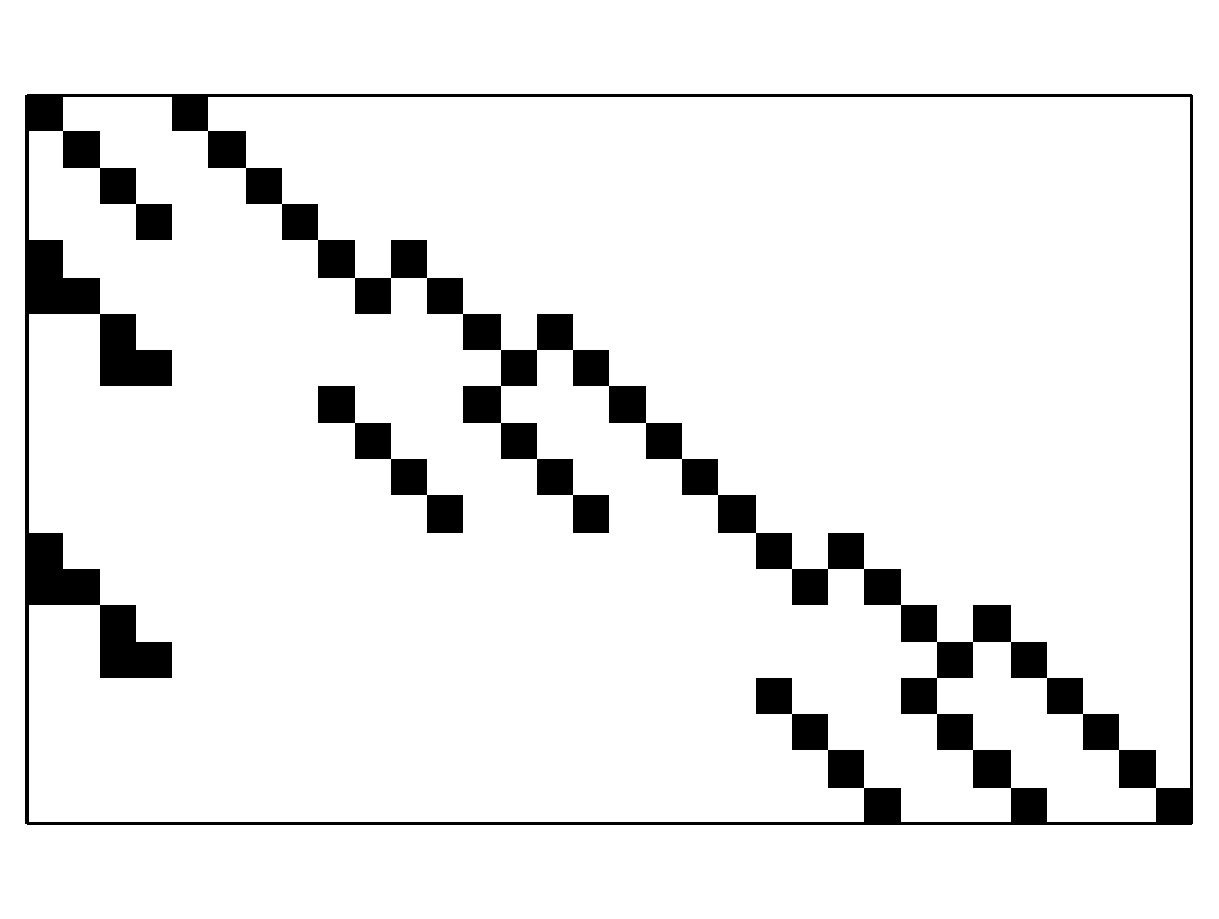
\includegraphics[width=0.45\linewidth]{DCAP_2_2_2_2}
		\label{fig:plotall_b}
	}
	
	\subfloat[][DCAP\_2\_2\_2\_2\_block\_T.pdf]
	{
		\centering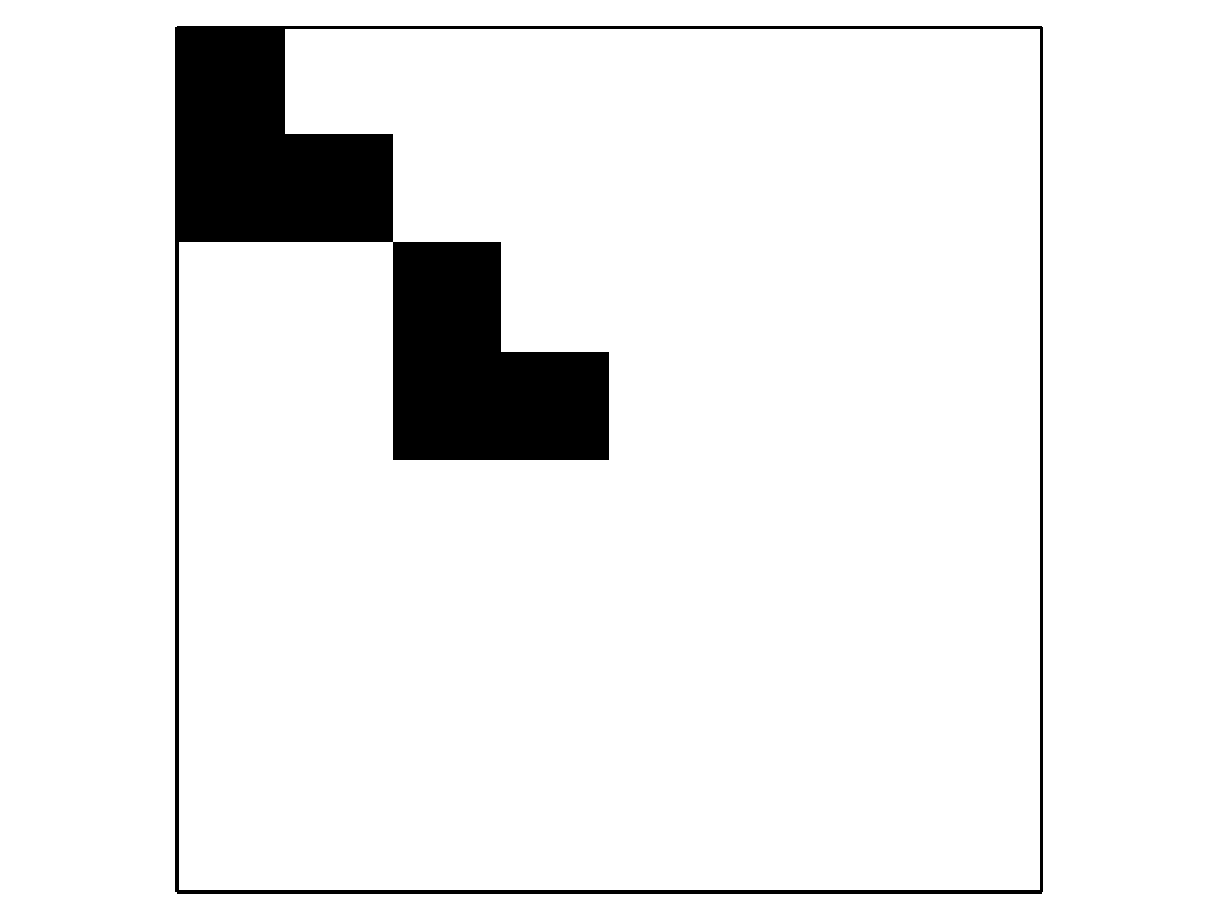
\includegraphics[width=0.45\linewidth]{DCAP_2_2_2_2_block_T}
		\label{fig:plotall_c}
	}
	~
	\subfloat[][DCAP\_2\_2\_2\_2\_block\_W.pdf]
	{
		\centering
\includegraphics[width=0.45\linewidth]{DCAP_2_2_2_2_block_W}
		\label{fig:plotall_d}
	}
	
	\caption{Plots drawn by executing function \texttt{plotAll}}
	%	\begin{minipage}
	%	\end{minipage}
	\label{fig:plotall}
\end{figure}
By executing \texttt{plotAll()}, one can obtain all the plots in Fig. \ref{fig:plotall}.

%\kk{This subsection can probably be removed from the paper and should go to a manual or a repository. Otherwise, please describe why/how this can be used for research.}
%\yoc{I move this to appendix. We can remove this.}

%
%\subsection{Solving instances: interfacing with \texttt{DSP} solver}
%\subsubsection{Extensive form: Invoking standard MIP solver}
%
%\subsubsection{Dual decomposition}
%
%\subsubsection{Benders decomposition}

